\documentclass[a4paper,11pt]{exam}
\printanswers % pour imprimer les réponses (corrigé)
%\noprintanswers % Pour ne pas imprimer les réponses (énoncé)
\addpoints % Pour compter les points
% \noaddpoints % pour ne pas compter les points
%\qformat{\textbf{\thequestion ) } }
%\qformat{\textbf{\thequestion )}} % Pour définir le style des questions (facultatif)
\usepackage{color} % définit une nouvelle couleur
\shadedsolutions % définit le style des réponses
% \framedsolutions % définit le style des réponses
\definecolor{SolutionColor}{rgb}{0.8,0.9,1} % bleu ciel
\renewcommand{\solutiontitle}{\noindent\textbf{Solution:}\par\noindent} % Définit le titre des solutions




\makeatletter

\def\maketitle{{\centering%
	\par{\huge\textbf{\@title}}%
	\par{\@date}%
	\par}}


\renewcommand{\thesubsection}{\Alph{subsection}.}   

\makeatother

\lhead{NOM Pr\'enom :}
\rhead{\textbf{Les r\'eponses doivent \^etre justifi\'ees et r\'edig\'ees}}
\cfoot{\thepage / \pageref{LastPage}}


%\usepackage{../../pas-math}
%\usepackage{../../moncours}


%\usepackage{pas-cours}
%-------------------------------------------------------------------------------
%          -Packages nécessaires pour écrire en Français et en UTF8-
%-------------------------------------------------------------------------------
\usepackage[utf8]{inputenc}
\usepackage[frenchb]{babel}
%\usepackage{numprint}
\usepackage[T1]{fontenc}
%\usepackage{lmodern}
\usepackage{textcomp}
\usepackage[french, boxed]{algorithm2e}
\usepackage{hyperref}


%-------------------------------------------------------------------------------

%-------------------------------------------------------------------------------
%                          -Outils de mise en forme-
%-------------------------------------------------------------------------------
\usepackage{hyperref}
\hypersetup{pdfstartview=XYZ}
%\usepackage{enumerate}
\usepackage{graphicx}
\usepackage{multicol}
\usepackage{tabularx}
\usepackage{multirow}
\usepackage{color}
\usepackage{eurosym}


\usepackage{anysize} %%pour pouvoir mettre les marges qu'on veut
%\marginsize{2.5cm}{2.5cm}{2.5cm}{2.5cm}

\usepackage{indentfirst} %%pour que les premier paragraphes soient aussi indentés
\usepackage{verbatim}
\usepackage{enumitem}
\usepackage{booktabs}
\usepackage[usenames,dvipsnames,svgnames,table]{xcolor}

\usepackage{variations}

%-------------------------------------------------------------------------------


%-------------------------------------------------------------------------------
%                  -Nécessaires pour écrire des mathématiques-
%-------------------------------------------------------------------------------
\usepackage{amsfonts}
\usepackage{amssymb}
\usepackage{amsmath}
\usepackage{amsthm}
\usepackage{tikz}
\usepackage{xlop}
\usepackage[output-decimal-marker={,}]{siunitx}
%-------------------------------------------------------------------------------

%-------------------------------------------------------------------------------
%                  -Nécessaires pour écrire des formules chimiquess-
%-------------------------------------------------------------------------------

\usepackage[version=4]{mhchem}

%-------------------------------------------------------------------------------
% Pour pouvoir exploiter les fichiers directement dans beamer
\newcommand{\pause}{\ }
%-------------------------------------------------------------------------------
%                    - Mise en forme avancée
%-------------------------------------------------------------------------------

\usepackage{ifthen}
\usepackage{ifmtarg}


\newcommand{\ifTrue}[2]{\ifthenelse{\equal{#1}{true}}{#2}{$\qquad \qquad$}}

%\newcommand{\kword}[1]{\textcolor{red}{\underline{#1}}}
%-------------------------------------------------------------------------------

%-------------------------------------------------------------------------------
%                     -Mise en forme d'exercices-
%-------------------------------------------------------------------------------
%\newtheoremstyle{exostyle}
%{\topsep}% espace avant
%{\topsep}% espace apres
%{}% Police utilisee par le style de thm
%{}% Indentation (vide = aucune, \parindent = indentation paragraphe)
%{\bfseries}% Police du titre de thm
%{.}% Signe de ponctuation apres le titre du thm
%{ }% Espace apres le titre du thm (\newline = linebreak)
%{\thmname{#1}\thmnumber{ #2}\thmnote{. \normalfont{\textit{#3}}}}% composants du titre du thm : \thmname = nom du thm, \thmnumber = numéro du thm, \thmnote = sous-titre du thm

%\theoremstyle{exostyle}
%\newtheorem{exercice}{Exercice}
%
%\newenvironment{questions}{
%\begin{enumerate}[\hspace{12pt}\bfseries\itshape a.]}{\end{enumerate}
%} %mettre un 1 à la place du a si on veut des numéros au lieu de lettres pour les questions 
%-------------------------------------------------------------------------------

%-------------------------------------------------------------------------------
%                    - Mise en forme de tableaux -
%-------------------------------------------------------------------------------

\renewcommand{\arraystretch}{1.7}

\setlength{\tabcolsep}{1.2cm}

%-------------------------------------------------------------------------------



%-------------------------------------------------------------------------------
%                    - Racourcis d'écriture -
%-------------------------------------------------------------------------------
%Droites
\newcommand{\dte}[1]{$(#1)$}
\newcommand{\fig}[1]{figure $#1$}
\newcommand{\sym}{symétrique}
\newcommand{\syms}{symétriques}
\newcommand{\asym}{axe de symétrie}
\newcommand{\asyms}{axes de symétrie}
\newcommand{\seg}[1]{$[#1]$}
\newcommand{\monAngle}[1]{$\widehat{#1}$}
\newcommand{\bissec}{bissectrice}
\newcommand{\mediat}{médiatrice}
\newcommand{\ddte}[1]{$[#1)$}


% Angles orientés (couples de vecteurs)
\newcommand{\aopp}[2]{(\vec{#1}, \vec{#2})} %Les deuc vecteurs sont positifs
\newcommand{\aopn}[2]{(\vec{#1}, -\vec{#2})} %Le second vecteur est négatif
\newcommand{\aonp}[2]{(-\vec{#1}, \vec{#2})} %Le premier vecteur est négatif
\newcommand{\aonn}[2]{(-\vec{#1}, -\vec{#2})} %Les deux vecteurs sont négatifs

%Ensembles mathématiques
\newcommand{\naturels}{\mathbb{N}} %Nombres naturels
\newcommand{\relatifs}{\mathbb{Z}} %Nombres relatifs
\newcommand{\rationnels}{\mathbb{Q}} %Nombres rationnels
\newcommand{\reels}{\mathbb{R}} %Nombres réels
\newcommand{\complexes}{\mathbb{C}} %Nombres complexes


%Intégration des parenthèses aux cosinus
\newcommand{\cosP}[1]{\cos\left(#1\right)}
\newcommand{\sinP}[1]{\sin\left(#1\right)}


%Probas stats
\newcommand{\stat}{statistique}
\newcommand{\stats}{statistiques}


\newcommand{\homo}{homothétie}
\newcommand{\homos}{homothéties}


\newcommand{\mycoord}[3]{(\textcolor{red}{\num{#1}} ; \textcolor{Green}{\num{#2}} ; \textcolor{blue}{\num{#3}})}
%-------------------------------------------------------------------------------

%-------------------------------------------------------------------------------
%                    - Mise en page -
%-------------------------------------------------------------------------------

\newcommand{\twoCol}[1]{\begin{multicols}{2}#1\end{multicols}}


\setenumerate[1]{font=\bfseries,label=\textit{\alph*})}
\setenumerate[2]{font=\bfseries,label=\arabic*)}


%-------------------------------------------------------------------------------
%                    - Elements cours -
%-------------------------------------------------------------------------------

%Correction d'exercice
\newcommand{\exoSec}[2]{\subsection*{Exercice #1 page #2}}
%-------------------------------------------------------------------------------
%                    - raccourcis d'écriture -
%-------------------------------------------------------------------------------

%Mise en évidence de termes clés
\newcommand{\mykw}[1]{\textcolor{red}{\underline{\textbf{#1}}}}

%Exercices
\newcommand{\exo}[2]{exercice #1 page #2}
\newcommand{\Exo}[2]{Exercice #1 page #2}

\renewcommand{\pause}{\ }

%Intervalles
\newcommand{\interOO}[2]{$]$#1 , #2$[$}
\newcommand{\interOF}[2]{$]$#1 , #2$]$}
\newcommand{\interFO}[2]{$[$#1 , #2$[$}
\newcommand{\interFF}[2]{$[$#1 , #2$]$}



%\usepackage{fullpage}
\author{\ }
\date{15 Février 2019}
\title{Sciences Physiques : DS n° 3}


\begin{document}
%	\usepackage{fancyhdr}
%	
%	\pagestyle{fancy}
%	\fancyhf{}
	%\rhead{Share\LaTeX}


	\maketitle


\begin{small}
	\begin{center}
		\begin{tabular}{|@{\ }l@{}|@{\ }c@{\ }|}
			\hline
			\textbf{Compétence} & \textbf{Maitrise} \\
			\hline
			 Exploiter les lois de l’électricité. \ \ &  \ \ \ \\
			\hline
			Dipôles en série, dipôles en dérivation. &  \\
			\hline			
			Mettre en oeuvre des tests caractéristiques d’espèces chimiques à partir d’une banque fournie.  &  \\
			\hline
			
		\end{tabular}
	\end{center}
\end{small}	
%	

Le soin et la qualité de rédaction sont pris en compte dans la notation.
Seul l'\ref{ex_schema} est à traiter sur le sujet, les autres se font sur la copie.

\vspace*{-0.5cm}
%\section{Orbite de la Terre (4 points)}

La Terre tourne autour du Soleil à une distance moyenne d'environ 150 millions de kilomètres suivant une période de \num{365.25} jours. On considère que le mouvement de la Terre autour du Soleil est circulaire.

\begin{center}
	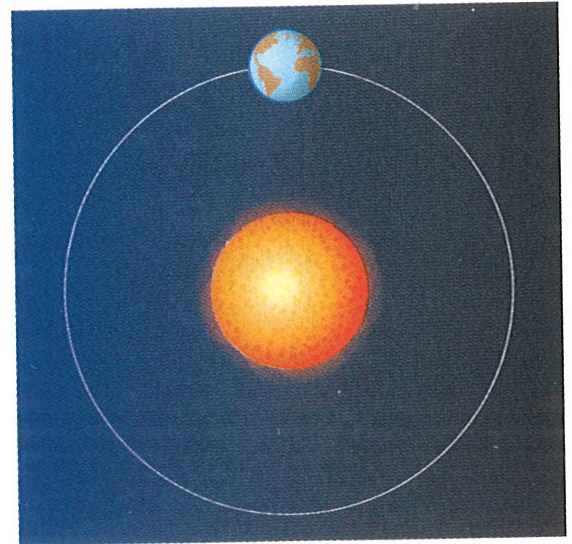
\includegraphics[scale=0.5]{terre}
\end{center}

\begin{questions}
	\question[2] Quelle est la distance parcourue par la Terre autour du Soleil pendant une année ?
	\fillwithdottedlines{3cm}
	
	\question[2] Calculer la vitesse de rotation de la Terre en km/h puis en km/s.
	\fillwithdottedlines{3cm}
\end{questions}


\section{Phrases à compléter (3 points)}

Recopier et compléter les phrases suivantes :

\begin{questions}
	\question[\half] Dans un circuit, plus la résistance augmente, plus l'intensité du courant $....$ .
	\begin{solution}
		Dans un circuit, plus la résistance augmente, plus l'intensité du courant \textbf{diminue}.
	\end{solution}
	
	\question[1] La résistance électrique se mesure à l'aide d'un $....$ et s'exprime en $....$ .
	\begin{solution}
		La résistance électrique se mesure à l'aide d'un \textbf{ohmmètre} et s'exprime en \textbf{ohm} .
	\end{solution}
	
	\question[1\half] La tension aux bornes d'un conducteur ohmique est $....$ à l'intensité du courant qui le traverse : c'est la loi d'Ohm, que l'on traduit par la relation : $....$ = $R$ $\times$  $....$.
	
	\begin{solution}
		La tension aux bornes d'un conducteur ohmique est \textbf{proportionnelle} à l'intensité du courant qui le traverse : c'est la loi d'Ohm, que l'on traduit par la relation : $\mathbf{U}$ = $R$ $\times$  $\mathbf{I}$.
	\end{solution}
\end{questions}

\section{Schema (2 points)}\label{ex_schema}

Compléter le schéma suivant :

\begin{center}
	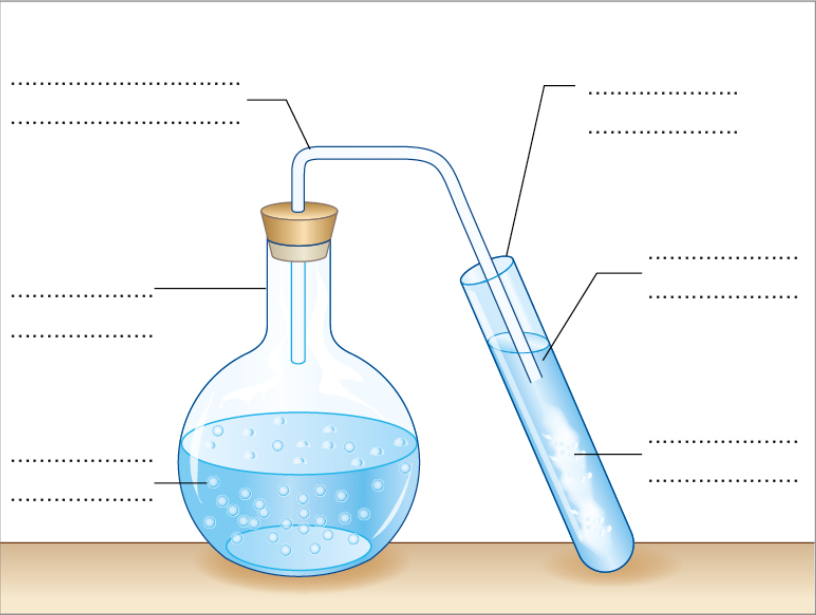
\includegraphics[scale=0.7]{img/gaz}
\end{center}

\begin{solution}
	\begin{center}
		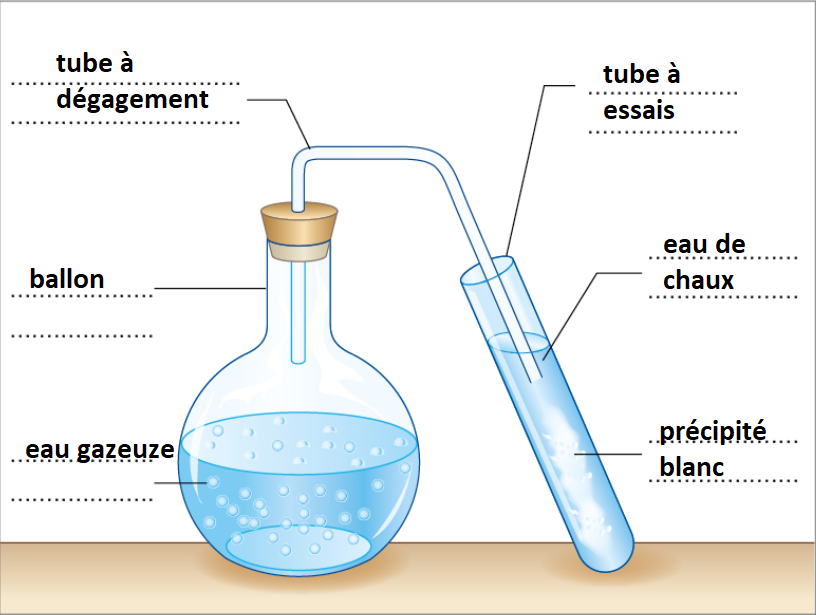
\includegraphics[scale=0.5]{img/gaz_2}
	\end{center}
\end{solution}

\section{Branches et n\oe uds (4 points)}

\begin{questions}
	\question Tracer le schéma normalisé du circuit ci-dessous.
	\question Surligne en rouge la branche principale, et d'une autre couleur les branches dérivées.
	
	\question Indique les n\oe uds.
\end{questions}

\begin{center}
	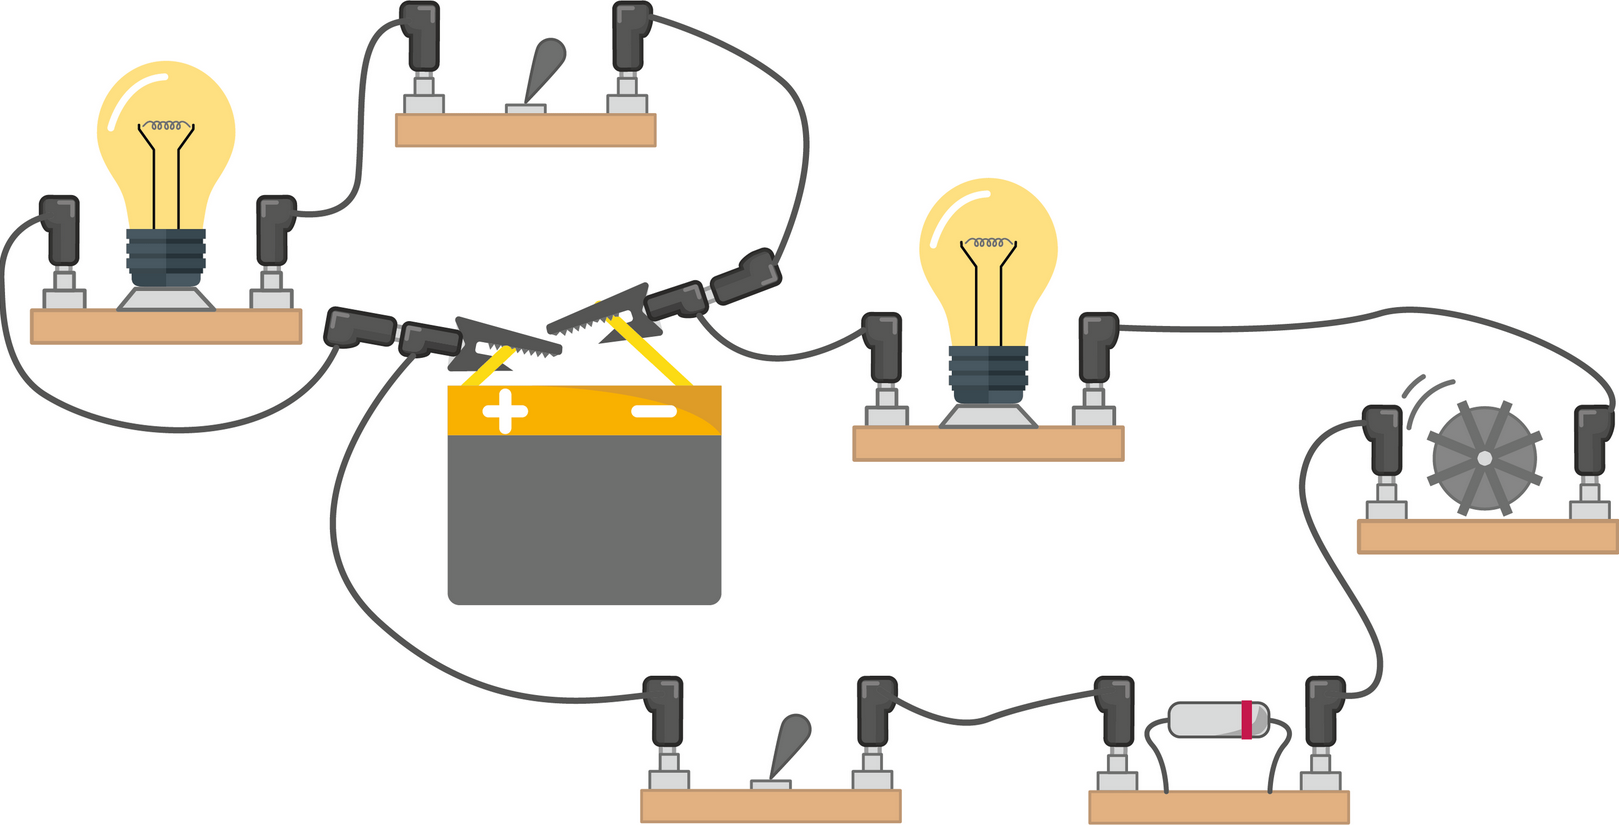
\includegraphics[scale=0.3]{img/ex18}
\end{center}

\begin{solution}
	\begin{center}
		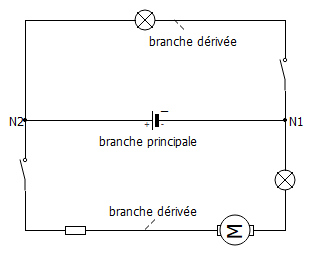
\includegraphics[scale=1.1]{img/ex3_exam}
	\end{center}
\end{solution}

\section{Circuit série et intensité (4 points)}

\begin{questions}
	\question Trace le schéma normalisé du circuit ci-dessous. Repère les intensités $I_1$ à $I_4$ qui sont mesurées par les ampèremètres $A_1$ à $A_4$.
	
	\question L'ampèremètre $A_3$ mesure une intensité $I_3$ de \num{0.250} A. Que valent $I_1$, $I_2$ et $I_4$.
\end{questions}

\begin{center}
	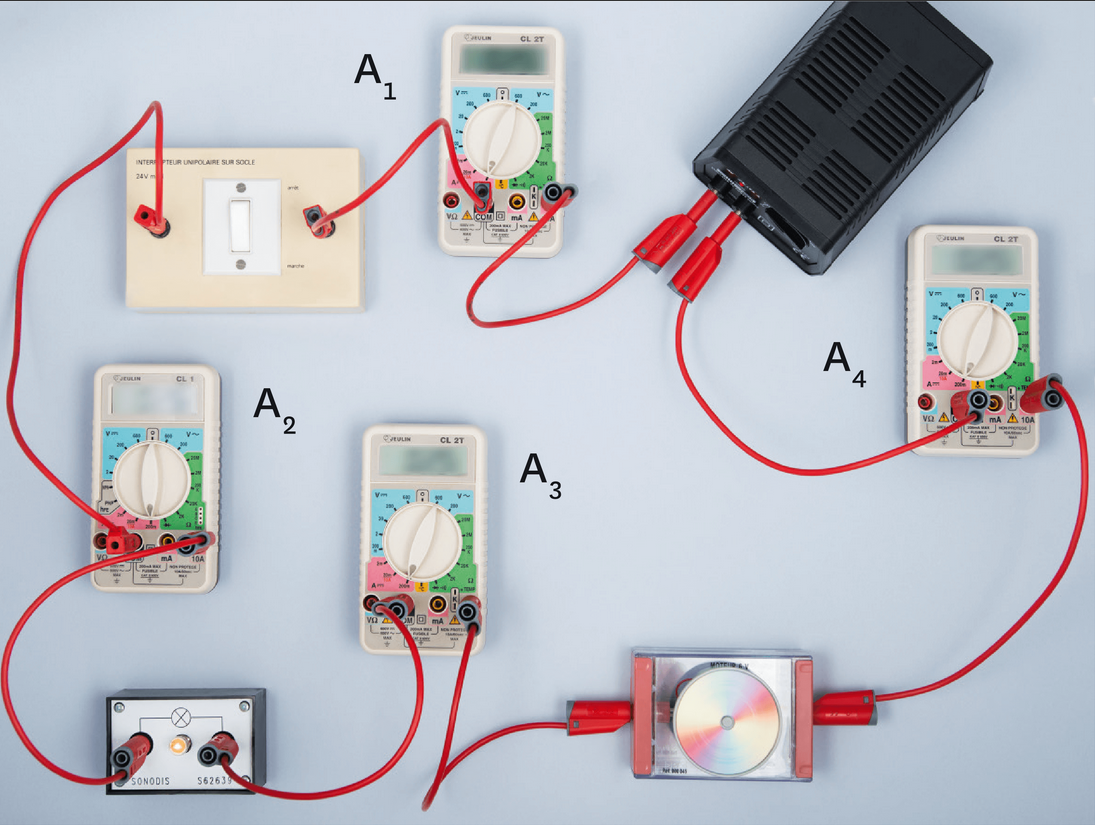
\includegraphics[scale=0.4]{img/ex15}
\end{center}


\newpage

\section{Résolution d'un problème (4 points)}

Par mégarde, on a remplacé un fusible de 5 $A$ par un fusible de 10 $A$ dans le tableau électrique de la voiture. Qu'a-t-il pu arriver à la voiture Tesla pour qu'elle prenne feu ?


	\begin{doc}[h!]
		\caption{Voiture électrique Tesla S\textregistered}
		
		\begin{center}
			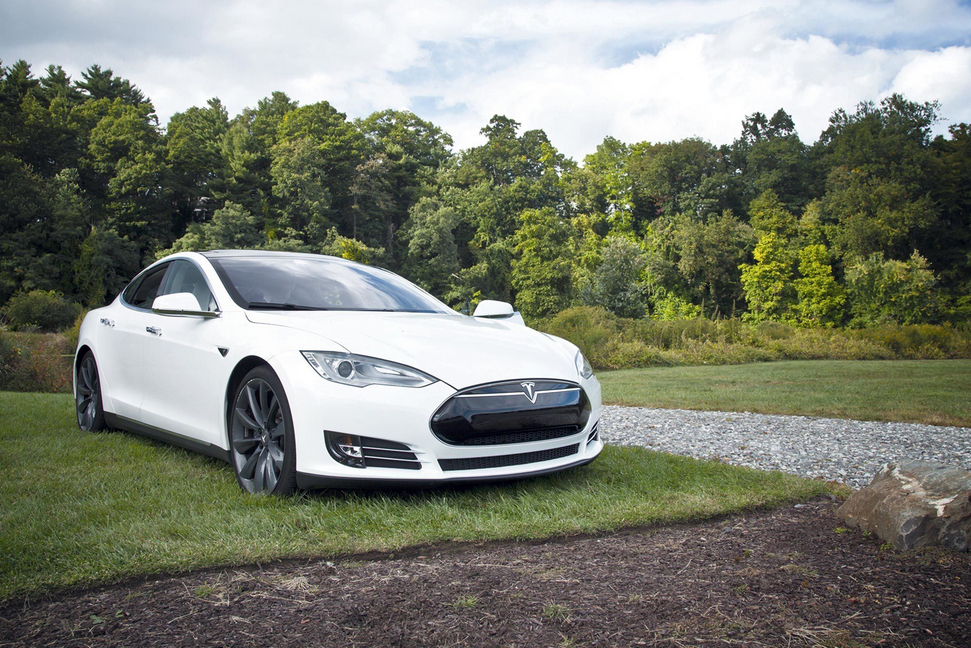
\includegraphics[scale=0.35]{img/tesla}
		\end{center}
	\end{doc}
	
	\begin{doc}[h!]
		\caption{D'après l'Est Républicain, 17 aout 2016 }
		
		<< Une voiture du fabricant américain de véhicules électriques Tesla Motors (modèle S90 D) a pris feu spontanément ce lundi à Bayonne à l'occasion de journées promotionnelles.>>
	\end{doc}




\begin{doc}[h!]
	\caption{Schéma de différents fusibles à lames}
	
	\begin{center}
		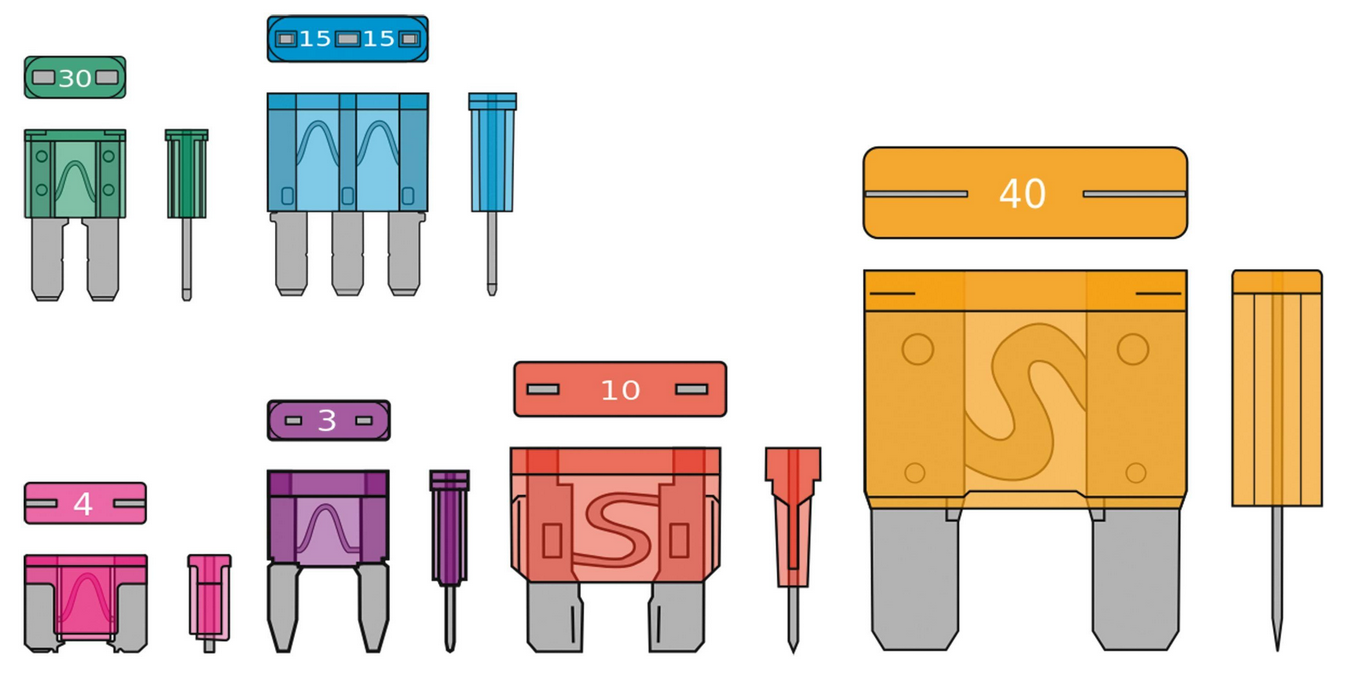
\includegraphics[scale=0.3]{img/fusibles}
	\end{center}
	
	Pour protéger les circuits électriques des véhicules, on utilise des fusibles. Ceux-cis fondent en cas d'intensité trop forte : le circuit est alors ouvert.
\end{doc}

\begin{solution}
	La voiture a pris feu à cause d'une surintensité, une partie de son circuit électrique a été traversée par un courant d'une intensité supérieure à celle prévue à cause d'un mauvais fusible.
	Si le courant a une intensité supérieure à 5 $A$ le fusible est censé fondre et ouvrir le circuit pour empêcher les problèmes. Mais ce fusible a été remplacé par un de 10 $A$, il n'a donc pas fondu.
\end{solution}

\newpage

\section{Romain et le sapin de Noël (3 points)}

%\begin{multicols}{2}
	Romain a un mini sapin de Noël qui décoré de trois guirlandes lumineuses alimentées par une pile. Il mesure les intensités sans le circuit mais son ampèremètre tombe en panne avant qu'il n'ait pu mesurer l'intensité $I_3$ qui traverse la guirlande bleue.
	
	\begin{questions}
		\question Comment peut-il faire pour déterminer $I_3$ sans la mesurer ? 
		\question Quelle valeur trouvera-t-il ?
	\end{questions}

\textbf{Données : } $I_1 = 450 mA$, $I_2 = 450 mA$, $I_4 = 125 mA$

\begin{center}
	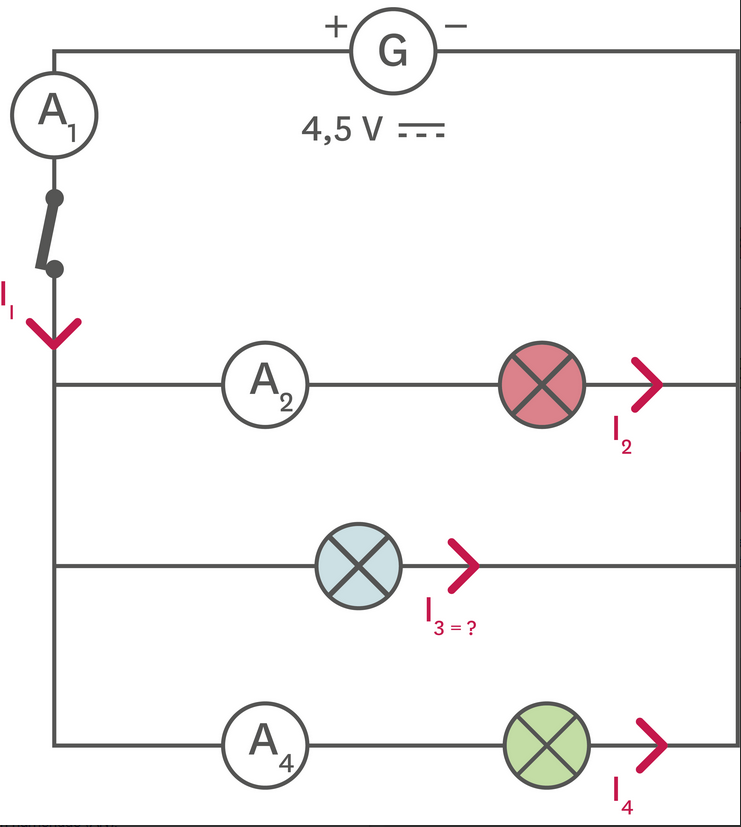
\includegraphics[scale=0.5]{img/sapin}
\end{center}
%\end{multicols}



\ \label{LastPage}

\end{document}